\chapter{Concurrency in C++}

\section{Threads}

\begin{paracol}{2}
   \begin{figure}[htbp]
      \centering
      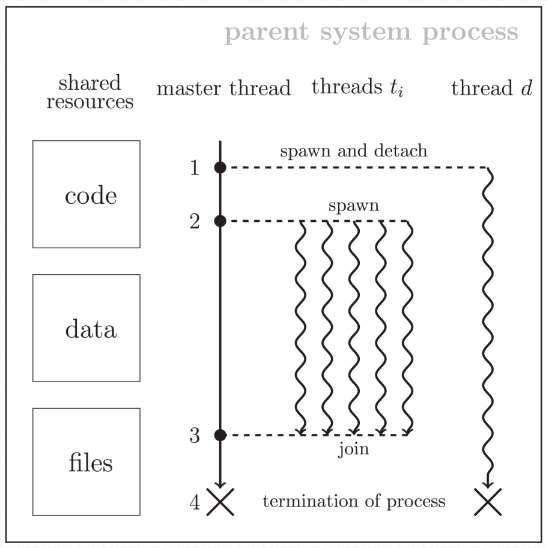
\includegraphics{images/08/threads1.png}
      \caption{Thread schema}
      \label{fig:08/threads1}
   
   \end{figure}
   
   \switchcolumn
   
   \begin{itemize}
      \item The master thread can spawn threads, and each thread can
   spawn threads as well
      \item The number of spawned threads should be roughly the
   amount of cores (i.e., pay attention to oversubscription)
      \item Threads share process resources
      \item each thread has a separate stack
      \item A thread can be joined or detached once
      \item A detached thread cannot be joined
      \item Joined or detached threads cannot be reused
      \item All threads must be joined or detached within the scope of
   their declaration
   \end{itemize}
\end{paracol}

\begin{itemize}
	\item We need to store the thread handles explicitly to be able
to access them during the join phase
	\item In the code snippet, we use a std::vector container and
the method emplace_back
	\item Alternatively, we could have moved the thread object
implicitly using the vector member function push_back
	\item \lstinline|threads.push_back(std :: thread(say_hello, id));|
	\item The type std::thread is move-only (i.e., not copyable)
	\item How to compile:
	\item \lstinline|g++ -O2 -std=c++17 hello_world.cpp -o hello_world -pthread|
\end{itemize}

